\def\curso{Tercero medio}
\def\titulo{Guía}
\def\subtitulo{Unidad de álgebra y funciones}
\documentclass[sin nombre]{srs}

\begin{document}
\section{Función afín}
\begin{preguntas}[after-item-skip=2cm]
\pregunta ¿Cuál es el punto de intersección de las diagonales del rectángulo cuyos vértices tienen coordenadas $\left(1,\,4\right)$, $\left(-3,\,4\right)$, $\left(-3,\,-4\right)$ y $\left(1,\,-4\right)$?
\begin{vertical}
\alternativa $\left(-3,\,0\right)$
\alternativa $\left(-2,\,0\right)$
\alternativa $\left(-1,\,0\right)$
\alternativa $\left(0,\,-1\right)$
\alternativa $\left(0,\,-2\right)$
\end{vertical}

\pregunta Si los puntos $P\left(4,\,-2\right)$, $Q\left(4,\,6\right)$ y $R\left(1,\,2\right)$ son los vértices de un triángulo, entonces el perímetro de este es
\begin{vertical}
\alternativa 5
\alternativa 12
\alternativa 18
\alternativa 21
\alternativa 24
\end{vertical}

\pregunta ¿Cuál debe ser el valor de $a$ en el punto $C$ para que los puntos $A\left(2,\,5\right)$, $B\left(-1,\,-4\right)$ y $C\left(a,\,-10\right)$ sean colineales?
\begin{vertical}
\alternativa $-3$
\alternativa $-5$
\alternativa $-6$
\alternativa $3$
\alternativa $1$
\end{vertical}

\pregunta ¿Cuál de las siguientes rectas tiene pendiente 6?
\begin{alternativasgraficas}
\alternativa \begin{tikzpicture}[scale=0.75]
  \draw [->] (-2.5,0) -- (2.5,0) node [right] {$x$};
  \draw [->] (0,-2.5) -- (0,2.5) node [above] {$y$};
  \draw[shorten >=-20pt, shorten <=-20pt] (-1.5,0) node [below] {$-6$} -- (0,1) node [right] {1};
\end{tikzpicture}
\alternativa \begin{tikzpicture}[scale=0.75]
  \draw [->] (-2.5,0) -- (2.5,0) node [right] {$x$};
  \draw [->] (0,-2.5) -- (0,2.5) node [above] {$y$};
  \draw[shorten >=-20pt, shorten <=-20pt] (-1,0) node [below] {$-1$} -- (0,1.5) node [right] {6};
\end{tikzpicture}
\alternativa \begin{tikzpicture}[scale=0.75]
  \draw [->] (-2.5,0) -- (2.5,0) node [right] {$x$};
  \draw [->] (0,-2.5) -- (0,2.5) node [above] {$y$};
  \draw[shorten >=-20pt, shorten <=-20pt] (0,-1) node [left] {$-1$} -- (1.5,0) node [below] {6};
\end{tikzpicture}
\alternativa \begin{tikzpicture}[scale=0.75]
  \draw [->] (-2.5,0) -- (2.5,0) node [right] {$x$};
  \draw [->] (0,-2.5) -- (0,2.5) node [above] {$y$};
  \draw[shorten >=-20pt, shorten <=-20pt] (0,1) node [left] {$1$} -- (1.5,0) node [below] {6};
\end{tikzpicture}
\alternativa \begin{tikzpicture}[scale=0.75]
  \draw [->] (-2.5,0) -- (2.5,0) node [right] {$x$};
  \draw [->] (0,-2.5) -- (0,2.5) node [above] {$y$};
  \draw[shorten >=-20pt, shorten <=-20pt] (0,1.5) node [left] {6} -- (0.7,0) node [below] {1};
\end{tikzpicture}

\end{alternativasgraficas}

\pregunta ¿Cuál es el valor del parámetro $k$ en la recta $\left(k - 2\right)x + 2ky - 5 = 0$ para que sea paralela a la recta $3x + 2y - 7 = 0$?
\begin{vertical}
\alternativa $-1$
\alternativa $-4$
\alternativa $\dfrac{1}{2}$
\alternativa $1$
\alternativa $5$
\end{vertical}

\pregunta Si el punto $\left(k + 1,\, k - 3\right)$ pertenece a la recta $3x - 2y + 4 = 0$, entonces $k =$
\begin{vertical}
\alternativa $7$
\alternativa $3$
\alternativa $1$
\alternativa $-3$
\alternativa $-13$
\end{vertical}

\pregunta ¿Cuál(es) de las siguientes afirmaciones es (son) verdadera(s) con respecto a la recta $3x - 5y - 12 = 0$?
\begin{verticali}
\alternativa La recta intersecta al eje de las abscisas en el punto $\left(4, 0\right)$.
\alternativa La pendiente de la recta es positiva.
\alternativa La recta intersecta al eje de las ordenadas en el punto $\left(0, -12\right)$.
\end{verticali}
\begin{vertical}
\alternativa Solo I
\alternativa Solo II
\alternativa Solo I y II
\alternativa Solo II y III
\alternativa I, II y III
\end{vertical}

\pregunta ¿Cuál es la ecuación de la recta que pasa por el punto $\left(-7, 2\right)$ y es perpendicular a la recta que une los puntos $\left(2,1\right)$ y $\left(-3,-3\right)$?
\begin{vertical}
\alternativa $5x + 4y + 27 = 0$
\alternativa $4x + 5y - 38 = 0$
\alternativa $4x + 5y + 18 = 0$
\alternativa $5x + 4y - 43 = 0$
\alternativa $5x + 4y + 38 = 0$
\end{vertical}

\pregunta ¿Cuál(es) de las siguientes afirmaciones es (son) verdadera(s) con respecto a la recta $L$ de la siguiente figura?
\begin{centrado}
\begin{tikzpicture}[scale=1.5]
  \draw [->] (-2,0) -- (1.5,0) node [right] {$x$};
  \draw [->] (0,-1) -- (0,2.5) node [above] {$y$};
  \draw[shorten >=-30pt, shorten <=-30pt] (-1,0) node [above,xshift=-7pt] {$-3$} -- (0,1.5) node [left] {6};
  \draw (0,0) --  ++(-7pt,0) -- ([turn]-90:7pt) -- ([turn]-90:7pt);
\end{tikzpicture}
\end{centrado}
\begin{verticali}
\alternativa La pendiente de la recta es 2.
\alternativa La ecuación de la recta es $y = 2x + 6$.
\alternativa El punto $\left(-5, -4\right)$ pertenece a la recta.
\end{verticali}
\begin{vertical}
\alternativa Sólo I
\alternativa Sólo II
\alternativa Sólo I y II
\alternativa Sólo II y III
\alternativa I, II y III
\end{vertical}


\pregunta Las rectas $L_1$ y $L_2$ son perpendiculares, $L_1$ tiene pendiente -2 y pasa por el punto $\left(4, -3\right)$ y $L_2$ pasa por el punto $\left(2,1\right)$. ¿Cuál es la abscisa del punto de intersección?
\begin{vertical}
\alternativa -2
\alternativa -1
\alternativa 0
\alternativa 1
\alternativa 2
\end{vertical}

\pregunta En cierta empresa de telefonía celular la relación entre la duración de una llamada, en minutos, y su valor es lineal. Si una llamada de 15 minutos cuesta \$ 770 y otra de 22 minutos cuesta \$ 1.120, ¿cuánto costará una llamada de 28 minutos?
\begin{vertical}
\alternativa \$ 773
\alternativa \$ 779
\alternativa \$ 1.290
\alternativa \$ 1.380
\alternativa \$ 1.420
\end{vertical}

\pregunta Se puede determinar el coeficiente de posición de una recta $L$, si:
\begin{verticaln}
\alternativa La recta $L$ corta al eje de las abscisas en el punto $\left(4,\,0\right)$.
\alternativa La recta $L$ forma con los ejes coordenados positivos un triángulo rectángulo de área 6.
\end{verticaln}
\begin{vertical}
\alternativa (1) por sí sola
\alternativa (2) por sí sola
\alternativa Ambas juntas, (1) y (2)
\alternativa Cada una por sí sola, (1) ó (2)
\alternativa Se requiere información adicional
\end{vertical}
\end{preguntas}

\section{Sistemas de ecuaciones}

\begin{preguntas}[after-item-skip=2cm]
\pregunta El par ordenado $\left(-4, 2\right)$ es solución del (de los) sistema(s):
\begin{tblr}{colspec={X[c]X[c]X[c]}}
I) $\begin{+cases} x + y = -2 \\ 2x + 5y = 2\end{+cases}$ &
II) $\begin{+cases} 3x - y = -14 \\ 7x + y = 14\end{+cases}$ &
III) $\begin{+cases} x + 2y = 0 \\ y = \dfrac{6-x}{5}\end{+cases}$ \\
\end{tblr}
\begin{vertical}
\alternativa Solo I
\alternativa Solo I y II
\alternativa Solo I y III
\alternativa Solo II y III
\alternativa I, II y III
\end{vertical}

\pregunta Para que el par ordenado $\left(2, 3\right)$ sea solución del sistema $\begin{+cases} px + y = 2 \\ x - qy = 5 \end{+cases}$, los valores de $p$ y $q$ deben ser respectivamente
\begin{vertical}
\alternativa $\dfrac{1}{2}$ y $1$
\alternativa $\dfrac{1}{2}$ y $-1$
\alternativa $-\dfrac{1}{2}$ y $-1$
\alternativa $-\dfrac{1}{2}$ y $1$
\alternativa $-2$ y $-1$
\end{vertical}

\pregunta La solución gráfica del sistema $\begin{+cases} 3x - 2y = 12 \\ 3x + y = 3 \end{+cases}$ es
\begin{alternativasgraficas}
\alternativa \begin{tikzpicture}[scale=1]
  \draw [->] (-0.5,0) -- (2,0) node [right] {$x$};
  \draw [->] (0,-2) -- (0,2) node [above] {$y$};
  \coordinate (A) at (0,-1.3);
  \coordinate (B) at (1.3,0);
  \draw[shorten >=-30pt, shorten <=-30pt] (A) node [left] {$-6$} -- (B) node [above] {4};
  %% cuadrado
  %%%\draw (0,0) --  ++(-7pt,0) -- ([turn]-90:7pt) -- ([turn]-90:7pt);
  %% punto destacado
  \coordinate (P) at ($(A)!.5!(B)$);
  \draw[dashed] (P) -- (P -| 0,0) node [left] {$-3$};
  \draw[dashed] (P) -- (P |- 0,0) node [above] {$2$};
  \fill (P) circle[radius=2pt];
  %% segunda recta
  \coordinate (C) at (0,1);
  \draw[shorten >=-30pt, shorten <=-20pt] (C) node [left] {$5$} -- (P);
\end{tikzpicture}
\alternativa 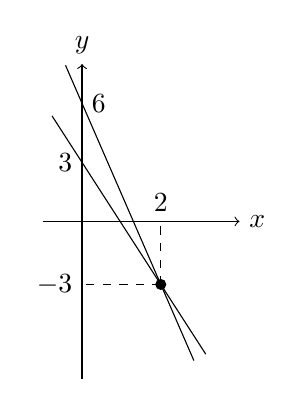
\begin{tikzpicture}[scale=1]
  \draw [->] (-0.5,0) -- (2,0) node [right] {$x$};
  \draw [->] (0,-2) -- (0,2) node [above] {$y$};
    %% punto destacado
  \coordinate (P) at (1,-0.8);
  \draw[dashed] (P) -- (P -| 0,0) node [left] {$-3$};
  \draw[dashed] (P) -- (P |- 0,0) node [above] {$2$};
  \fill (P) circle[radius=2pt];
  %% primera recta
  \coordinate (A) at (0,1.5);
  \coordinate (B) at (1.3,0);
  \draw[shorten >=-30pt, shorten <=-15pt] (A) node [right] {$6$} -- (P);
  %% cuadrado
  %%%\draw (0,0) --  ++(-7pt,0) -- ([turn]-90:7pt) -- ([turn]-90:7pt);
  %% segunda recta
  \coordinate (C) at (0,0.75);
  \draw[shorten >=-30pt, shorten <=-20pt] (C) node [left] {$3$} -- (P);
\end{tikzpicture}
\alternativa \begin{tikzpicture}[scale=1]
  \draw [->] (-0.5,0) -- (2,0) node [right] {$x$};
  \draw [->] (0,-2) -- (0,2) node [above] {$y$};
  \coordinate (A) at (0,-1.3);
  \coordinate (B) at (1.3,0);
  \draw[shorten >=-30pt, shorten <=-30pt] (A) node [left] {$-4$} -- (B) node [above] {6};
  %% cuadrado
  %%%\draw (0,0) --  ++(-7pt,0) -- ([turn]-90:7pt) -- ([turn]-90:7pt);
  %% punto destacado
  \coordinate (P) at ($(A)!.5!(B)$);
  \draw[dashed] (P) -- (P -| 0,0) node [left] {$-3$};
  \draw[dashed] (P) -- (P |- 0,0) node [above] {$2$};
  \fill (P) circle[radius=2pt];
  %% segunda recta
  \coordinate (C) at (0,1);
  \draw[shorten >=-30pt, shorten <=-20pt] (C) node [left] {$3$} -- (P);
\end{tikzpicture}
\alternativa \begin{tikzpicture}[scale=1]
  \draw [->] (-0.5,0) -- (2,0) node [right] {$x$};
  \draw [->] (0,-2) -- (0,2) node [above] {$y$};
  \coordinate (A) at (0,-1.3);
  \coordinate (B) at (1.3,0);
  \draw[shorten >=-30pt, shorten <=-30pt] (A) node [left] {$-6$} -- (B) node [above] {4};
  %% cuadrado
  %%%\draw (0,0) --  ++(-7pt,0) -- ([turn]-90:7pt) -- ([turn]-90:7pt);
  %% punto destacado
  \coordinate (P) at ($(A)!.5!(B)$);
  \draw[dashed] (P) -- (P -| 0,0) node [left] {$-3$};
  \draw[dashed] (P) -- (P |- 0,0) node [above] {$2$};
  \fill (P) circle[radius=2pt];
  %% segunda recta
  \coordinate (C) at (0,1);
  \draw[shorten >=-30pt, shorten <=-20pt] (C) node [left] {$3$} -- (P);
\end{tikzpicture}
\alternativa \begin{tikzpicture}[scale=1]
  \draw [->] (-0.5,0) -- (2,0) node [right] {$x$};
  \draw [->] (0,-2) -- (0,2) node [above] {$y$};
  \coordinate (A) at (0,-1.3);
  \coordinate (B) at (1.3,0);
  \draw[shorten >=-30pt, shorten <=-30pt] (A) node [left] {$-4$} -- (B) node [above] {6};
  %% cuadrado
  %%%\draw (0,0) --  ++(-7pt,0) -- ([turn]-90:7pt) -- ([turn]-90:7pt);
  %% punto destacado
  \coordinate (P) at ($(A)!.5!(B)$);
  \draw[dashed] (P) -- (P -| 0,0) node [left] {$-3$};
  \draw[dashed] (P) -- (P |- 0,0) node [above] {$2$};
  \fill (P) circle[radius=2pt];
  %% segunda recta
  \coordinate (C) at (0,0.5);
  \draw[shorten >=-30pt, shorten <=-20pt] (C) node [left] {$1$} -- (P);
\end{tikzpicture}

\end{alternativasgraficas}

\pregunta ¿Cuál de los siguientes sistemas tiene solución única?
\begin{vertical}
\alternativa $\begin{+cases} 2x + 5y = 4 \\ -6x - 15y = 12 \end{+cases}$
\alternativa $\begin{+cases} 2x + 2y = 4 \\ 3x - 3y = 1 \end{+cases}$
\alternativa $\begin{+cases} 3x + 9y = 4 \\ -6x - 18y = -8 \end{+cases}$
\alternativa $\begin{+cases} 3x + 9y = 4 \\ x + 3y = 1 \end{+cases}$
\alternativa $\begin{+cases} 2x + y = 4 \\ 4x + 2y = 8 \end{+cases}$
\end{vertical}

\pregunta ¿Cuál de los siguientes sistemas no tiene solución?
\begin{vertical}
\alternativa $\begin{+cases} 8x + 5y = 4 \\ 3x - 4y = 5 \end{+cases}$
\alternativa $\begin{+cases} x + y = 4 \\ x - y = 4 \end{+cases}$
\alternativa $\begin{+cases} -4x + 3y = -5 \\ 12x - 9y = -15 \end{+cases}$
\alternativa $\begin{+cases} 6x + 10y = 12 \\ -3x - 5y = -6 \end{+cases}$
\alternativa $\begin{+cases} 3x + 5y = -4 \\ 9x + 15y = -12 \end{+cases}$
\end{vertical}

\pregunta En el sistema $\begin{+cases} ax - 4 = by \\ 2x - 12 = 3y \end{+cases}$, ¿qué condición deben cumplir $a$ y $b$ para que tenga solución única?
\begin{vertical}
\alternativa $a \neq \dfrac{2}{3}$
\alternativa $3a \neq 2b$
\alternativa $3a = 2b$
\alternativa $3a = -2b$
\alternativa $3a \neq -2b$
\end{vertical}

\pregunta El enunciado: \q{El doble, de un número aumentado en 3 es igual a un segundo número, y la cuarta parte de su diferencia es 12}, está representado por
\begin{vertical}
\alternativa $\begin{+cases} 2x + 3 = y \\ \dfrac{x-y}{4} = 12 \end{+cases}$
\alternativa $\begin{+cases} 2\left(x + 3\right) = y \\ \dfrac{x-y}{4} = 12 \end{+cases}$
\alternativa $\begin{+cases} 2x - 3 = y \\ x - y = \dfrac{12}{4} \end{+cases}$
\alternativa $\begin{+cases} 2\left(x - 3\right) = y \\ x - y = 12 \cdot 4 \end{+cases}$
\alternativa $\begin{+cases} 2\left(x + 3\right) = y \\ \dfrac{x}{4} - y = 12 \end{+cases}$
\end{vertical}

\pregunta Un coleccionista compra dos antigüedades (A y B) por \$ 28.000 y las vende en \$ 30.000. Si por la venta de ambas, en A ganó el 30\% y por la otra perdió el 10\% sobre el precio de compra, ¿cuál es el sistema que permite determinar los precios de costos de cada antigüedad?
\begin{vertical}
\alternativa $\begin{+cases} A + B = 28.000 \\ 1,3A - 1,1B = 30.000 \end{+cases}$
\alternativa $\begin{+cases} A + B = 28.000 \\ 1,3A + 0,9B = 30.000 \end{+cases}$
\alternativa $\begin{+cases} A + B = 28.000 \\ 0,3A - 0,1B = 30.000 \end{+cases}$
\alternativa $\begin{+cases} A + B = 28.000 \\ 0,3A + 0,1B = 2.000 \end{+cases}$
\alternativa $\begin{+cases} A + B = 28.000 \\ 1,3A - 0,9B = 30.000 \end{+cases}$
\end{vertical}

\pregunta Juan con \$ 5.600 compra 20 lápices; unos que cuestan \$ 250 y otros que cuestan \$ 300. ¿Cuántos lápices de \$ 300 compró?
\begin{vertical}
\alternativa 2
\alternativa 8
\alternativa 12
\alternativa 18
\alternativa 20
\end{vertical}


\pregunta Dos números suman 42 y su diferencia es 12. ¿Cuáles son estos números?
\begin{vertical}
\alternativa $-27$~~y~~15
\alternativa 27~~y~~$-15$
\alternativa $-27$~~y~~$-15$
\alternativa 27~~y~~15
\alternativa 26~~y~~16
\end{vertical}

\pregunta Hallar el número de dos dígitos, tal que la suma de sus cifras es 9 y cuando se invierte el orden de sus cifras se obtiene un segundo número que excede en 9 al cuádruplo del número original.
\begin{vertical}
\alternativa 90
\alternativa 81
\alternativa 54
\alternativa 45
\alternativa 18
\end{vertical}

\pregunta Por la compra de 3 vacas y 7 terneros se paga \$ 480.000, mientras que por la compra de 7 vacas y 3 terneros se paga \$ 560.000. ¿Cuál es el costo de 5 vacas y 5 terneros?
\begin{vertical}
\alternativa \$ 1.040.000
\alternativa \$ 520.000
\alternativa \$ 104.000
\alternativa \$ 62.000
\alternativa \$ 42.000
\end{vertical}
\end{preguntas}

\section{Función cuadratica}

\begin{preguntas}[after-item-skip=2cm]
\pregunta ¿Cuál es la suma de las soluciones (o raíces) de la ecuación $7x^2 - 5x - 1 = 0$?
\begin{vertical}
\alternativa $-\dfrac{5}{7}$
\alternativa $-\dfrac{7}{5}$
\alternativa $\dfrac{1}{5}$
\alternativa $\dfrac{5}{7}$
\alternativa $\dfrac{1}{7}$
\end{vertical}

\pregunta ¿Cuál es el producto de las soluciones (o raíces) de la ecuación $5x^2 - 6x + 1 = 0$?
\begin{vertical}
\alternativa $-\dfrac{3}{5}$
\alternativa $-\dfrac{1}{5}$
\alternativa $\dfrac{1}{5}$
\alternativa $\dfrac{3}{5}$
\alternativa $\dfrac{6}{5}$
\end{vertical}

\pregunta Una ecuación de segundo grado cuyas raíces, $x_1$~~y~~$x_2$, satisfacen las igualdades $\left(x_1 + x_2\right) = -2$~~~y~~~$x_1 \cdot x_2 = 5$~~es
\begin{vertical}
\alternativa $x^2 - 2x - 5 = 0$
\alternativa $x^2 - 2x + 5 = 0$
\alternativa $x^2 + 2x + 5 = 0$
\alternativa $x^2 + 2x - 5 = 0$
\alternativa $x^2 - 5x - 2 = 0$
\end{vertical}

\pregunta ¿Cuál de las afirmaciones siguientes es correcta respecto a la parábola $y = -x^2 - 4x - 1$?
\begin{verticali}
\alternativa Intersecta al eje de las ordenadas en el punto $\left(0, -1\right)$
\alternativa Su concavidad es hacia arriba
\alternativa El punto $\left(-1, 2\right)$ pertenece a ella
\end{verticali}
\begin{vertical}
\alternativa Solo I
\alternativa Solo II
\alternativa Solo I y II
\alternativa Solo I y III
\alternativa I, II y III
\end{vertical}

\pregunta Con respecto de la función asociada al gráfico de la figura 2, ¿cuál(es) de las siguientes aseveraciones es (son) verdadera(s)?
\begin{centrado}
\begin{tikzpicture}[scale=1]
  \draw [->,name path=EjeX] (-2,0) -- (3,0) node [right] {$x$};
  \draw [->,name path=EjeY] (0,-2) -- (0,2) node [above] {$y$};
  %%% punto destacado
  %\coordinate (P) at ($(A)!.5!(B)$);
  %\draw[dashed] (P) -- (P -| 0,0) node [left] {$-3$};
  %\draw[dashed] (P) -- (P |- 0,0) node [above] {$2$};
  %\fill (P) circle[radius=2pt];
  %% curva
  \coordinate (A) at (-1,-1);
  \coordinate (B) at (2,-1);
  \draw[name path=Parabola] (A) parabola[bend pos=0.5] bend +(0,2) (B);
  \node[name intersections={of=EjeX and Parabola,name=I},above left] at (I-1) {$-2$};
  \node[name intersections={of=EjeX and Parabola,name=I},above right] at (I-2) {$5$};
\end{tikzpicture}
\end{centrado}
\begin{verticali}
\alternativa Tiene 2 ceros.
\alternativa El discriminante es mayor a cero.
\alternativa $f\left(0\right) = -2$
\end{verticali}
\begin{vertical}
\alternativa Solo III
\alternativa Solo I y II
\alternativa Solo I y III
\alternativa Solo II y III
\alternativa I, II y III
\end{vertical}

\pregunta Dada la función cuadrática $f\left(x\right) = x^2 + 2x - a$, es correcto afirmar que:
\begin{verticali}
\alternativa Si $a > -1$, existen 2 intersecciones con el eje x.
\alternativa Si $a = -1$, existe una intersección con el eje x.
\alternativa Si $a < -1$, no hay intersección con el eje x.
\end{verticali}
\begin{vertical}
\alternativa Solo I
\alternativa Solo II
\alternativa Solo I y II
\alternativa Solo II y III
\alternativa I, II y III
\end{vertical}

\pregunta El gráfico de la siguiente figura, podría corresponder a la función
\begin{centrado}
\begin{tikzpicture}[scale=1]
  \draw [->,name path=EjeX] (-3,0) -- (2,0) node [right] {$x$};
  \draw [->,name path=EjeY] (0,-1) -- (0,3) node [above] {$y$};
  %%% punto destacado
  %\coordinate (P) at ($(A)!.5!(B)$);
  %\draw[dashed] (P) -- (P -| 0,0) node [left] {$-3$};
  %\draw[dashed] (P) -- (P |- 0,0) node [above] {$2$};
  %\fill (P) circle[radius=2pt];
  %% curva
  \coordinate (A) at (-2,-0.5);
  \coordinate (B) at (1,-0.5);
  \draw[name path=Parabola] (A) parabola[bend pos=0.5] bend +(0,3) (B);
  \node[name intersections={of=EjeX and Parabola,name=I},above left] at (I-1) {$-3$};
  \node[name intersections={of=EjeX and Parabola,name=I},above right] at (I-2) {$1$};
\end{tikzpicture}
\end{centrado}
\begin{vertical}
\alternativa $f\left(x\right) = -x^2 + 2x - 3$
\alternativa $f\left(x\right) = -x^2 + 2x + 3$
\alternativa $f\left(x\right) = -x^2 - 2x - 3$
\alternativa $f\left(x\right) = -x^2 - 2x + 3$
\alternativa $f\left(x\right) = -x^2 - 3x + 4$
\end{vertical}

\pregunta La función cuadrática cuya parábola tiene vértice $\left(2, -3\right)$ es
\begin{vertical}
\alternativa $g = \left(x + 2\right)^2 + 3$
\alternativa $g = \left(x - 2\right)^2 + 3$
\alternativa $g = 3\left(x - 2\right)^2 - 3$
\alternativa $g = 3\left(x + 2\right)^2 - 3$
\alternativa $g = 3\left(x + 2\right)^2 + 3$
\end{vertical}

\pregunta Con respecto a la función cuadrática $f\left(x\right) = -2\left(x + 1\right)^2 + 2$, ¿cuál de las siguientes afirmaciones es (son) verdadera(s)?
\begin{verticali}
\alternativa Su vértice es $\left(-1, 2\right)$.
\alternativa Su eje de simetría es $x = -1$.
\alternativa Intersecta al eje de las ordenadas en el punto $\left(0, 0\right)$.
\end{verticali}
\begin{vertical}
\alternativa Solo I
\alternativa Solo II
\alternativa Solo I y II
\alternativa Solo I y III
\alternativa I, II y III
\end{vertical}

\pregunta Si $f\left(x\right) = \left(x - 3\right)^2 + 2$, su gráfico corresponde a
\begin{alternativasgraficas}
\alternativa
\begin{tikzpicture}[scale=1]
  \draw [->,name path=EjeX] (-2,0) -- (3,0) node [right] {$x$};
  \draw [->,name path=EjeY] (0,-1) -- (0,2) node [above] {$y$};
  %% curva
  \coordinate (A) at (-1,-0.5);
  \coordinate (B) at (2.5,-0.5);
  \draw[name path=Parabola] (A) parabola[bend pos=0.5] bend +(0,1.5) (B);
  \node[name intersections={of=EjeX and Parabola,name=I},above left] at (I-1) {$-1$};
  \node[name intersections={of=EjeX and Parabola,name=I},above right] at (I-2) {$7$};
    %%% punto destacado
  \path[name path=EjeSimetria] ($(A)!0.5!(B)$) -- +(0,3);
  \fill[name intersections={of=EjeSimetria and Parabola,by=V}] (V) circle[radius=2pt];
  \draw[dashed] (V) -- (V -| 0,0) node [left] {$2$};
  \draw[dashed] (V) -- (V |- 0,0) node [below] {$3$};

\end{tikzpicture}
\alternativa
\begin{tikzpicture}[scale=1]
  \draw [->,name path=EjeX] (-2,0) -- (3,0) node [right] {$x$};
  \draw [->,name path=EjeY] (0,-1) -- (0,2) node [above] {$y$};
  %% curva
  \coordinate (A) at (-0.2,-0.5);
  \coordinate (B) at (2.5,-0.5);
  \draw[name path=Parabola] (A) parabola[bend pos=0.5] bend +(0,1.5) (B);
  %\node[name intersections={of=EjeX and Parabola,name=I},above left] at (I-1) {$-1$};
  \node[name intersections={of=EjeX and Parabola,name=I},above right] at (I-2) {$6$};
    %%% punto destacado
  \path[name path=EjeSimetria] ($(A)!0.5!(B)$) -- +(0,3);
  \fill[name intersections={of=EjeSimetria and Parabola,by=V}] (V) circle[radius=2pt];
  \draw[dashed] (V) -- (V -| 0,0) node [left] {$2$};
  \draw[dashed] (V) -- (V |- 0,0) node [below] {$3$};

\end{tikzpicture}
\alternativa
\begin{tikzpicture}[scale=1]
  \draw [->,name path=EjeX] (-2,0) -- (3,0) node [right] {$x$};
  \draw [->,name path=EjeY] (0,-1) -- (0,2) node [above] {$y$};
  %% curva
  \coordinate (A) at (-0.2,2);
  \coordinate (B) at (2.8,2);
  \draw[name path=Parabola] (A) parabola[bend pos=0.5] bend +(0,-1.5) (B);
  %\node[name intersections={of=EjeX and Parabola,name=I},above left] at (I-1) {$-1$};
  %\node[name intersections={of=EjeX and Parabola,name=I},above right] at (I-2) {$6$};
  %%% punto destacado
  \path[name path=EjeSimetria] ($(A)!0.5!(B)$) -- +(0,-3);
  \fill[name intersections={of=EjeSimetria and Parabola,by=V}] (V) circle[radius=2pt];
  \draw[dashed] (V) -- (V -| 0,0) node [left] {$2$};
  \draw[dashed] (V) -- (V |- 0,0) node [below] {$3$};

\end{tikzpicture}
\alternativa
\begin{tikzpicture}[scale=1]
  \draw [->,name path=EjeX] (-3,0) -- (2,0) node [right] {$x$};
  \draw [->,name path=EjeY] (0,-1) -- (0,2) node [above] {$y$};
  %% curva
  \coordinate (A) at (-2.5,-0.5);
  \coordinate (B) at (0.5,-0.5);
  \draw[name path=Parabola] (A) parabola[bend pos=0.5] bend +(0,1.5) (B);
  \node[name intersections={of=EjeX and Parabola,name=I},above left] at (I-1) {$-7$};
  \node[name intersections={of=EjeX and Parabola,name=I},above right] at (I-2) {$1$};
    %%% punto destacado
  \path[name path=EjeSimetria] ($(A)!0.5!(B)$) -- +(0,3);
  \fill[name intersections={of=EjeSimetria and Parabola,by=V}] (V) circle[radius=2pt];
  \draw[dashed] (V) -- (V -| 0,0) node [right] {$2$};
  \draw[dashed] (V) -- (V |- 0,0) node [below] {$-3$};

\end{tikzpicture}
\alternativa
\begin{tikzpicture}[scale=1]
  \draw [->,name path=EjeX] (-2,0) -- (3,0) node [right] {$x$};
  \draw [->,name path=EjeY] (0,-1) -- (0,2) node [above] {$y$};
  %% curva
  \coordinate (A) at (0.2,-0.5);
  \coordinate (B) at (2.5,-0.5);
  \draw[name path=Parabola] (A) parabola[bend pos=0.5] bend +(0,1.5) (B);
  \node[name intersections={of=EjeX and Parabola,name=I},below right] at (I-1) {$1$};
  \node[name intersections={of=EjeX and Parabola,name=I},below left] at (I-2) {$5$};
    %%% punto destacado
  \path[name path=EjeSimetria] ($(A)!0.5!(B)$) -- +(0,3);
  \fill[name intersections={of=EjeSimetria and Parabola,by=V}] (V) circle[radius=2pt];
  \draw[dashed] (V) -- (V -| 0,0) node [left] {$2$};
  \draw[dashed] (V) -- (V |- 0,0) node [below] {$3$};

\end{tikzpicture}
\end{alternativasgraficas}

\pregunta La altura $h\left(t\right)$ alcanzada, medida en metros, de un proyectil se modela mediante la función $h\left(t\right) = 20t - 5t^{2}$, donde t es la cantidad de segundos que transcurren hasta que alcanza dicha altura. ¿Cuál(es) de las siguientes afirmaciones es (son) verdadera(s)?
\begin{verticali}
\alternativa A los 4 segundos llega al suelo.
\alternativa A los 2 segundos alcanza su altura máxima.
\alternativa Al primer y tercer segundo después de ser lanzado alcanza la misma altura.
\end{verticali}
\begin{vertical}
\alternativa Solo I
\alternativa Solo II
\alternativa Solo I y II
\alternativa Solo II y III
\alternativa I, II y III
\end{vertical}

\end{preguntas}

\end{document}
